%%%%%%%%%%%%%%%%%%%%%%%%%%%%%%%%%%%%%%%%%%%%%%%
% University Paderborn Beamer Presentation 

% Author: Ashwin Prasad Shivarpatna Venkatesh 

%This template is free: you can redistribute it and/or modify
%it under the terms of the GNU General Public License as published by
%the Free Software Foundation, either version 3 of the License, or any later version.
%
%This program is distributed in the hope that it will be useful,
%but WITHOUT ANY WARRANTY; without even the implied warranty of
%MERCHANTABILITY or FITNESS FOR A PARTICULAR PURPOSE.  See the
%GNU General Public License for more details.
%
%You should have received a copy of the GNU General Public License
%along with this program.  If not, see <https://www.gnu.org/licenses/>.

%%%%%%%%%%%%%%%%%%%%%%%%%%%%%%%%%%%%%%%%%%%%%%%

\documentclass{beamer}
% Default page size 12.8cm x 9.6cm

% import packages and user-defined commands
\usepackage{graphicx} % Allows including images
\usepackage{booktabs} % Allows the use of \toprule, \midrule and \bottomrule in tables
\usepackage{tikz}

\usepackage{helvet} % Font

\usepackage[english]{babel}
\usepackage{textcomp}
\usepackage{helvet} % Font
\usepackage{array}
\usepackage{listings}
\usepackage{color}
\usepackage{lstlinebgrd}
\usepackage{tikz}
\usetikzlibrary{shadows}
\definecolor{mygreen}{rgb}{0,0.6,0}
\definecolor{dkgreen}{rgb}{0,0.6,0}
\definecolor{gray}{rgb}{0.5,0.5,0.5}
\definecolor{mygray}{rgb}{0.5,0.5,0.5}
\definecolor{mymauve}{rgb}{0.58,0,0.82}

\lstset{ %
	language=[x86masm]Assembler,       % the language of the code
	basicstyle=\footnotesize,       % the size of the fonts that are used for the code
	numbers=left,                   % where to put the line-numbers
	numberstyle=\tiny\color{gray},  % the style that is used for the line-numbers
	stepnumber=1,                   % the step between two line-numbers. If it's 1, each line 
	% will be numbered
	numbersep=5pt,                  % how far the line-numbers are from the code
	backgroundcolor=\color{white},  % choose the background color. You must add \usepackage{color}
	showspaces=false,               % show spaces adding particular underscores
	showstringspaces=false,         % underline spaces within strings
	showtabs=false,                 % show tabs within strings adding particular underscores
	frame=single,                   % adds a frame around the code
	rulecolor=\color{black},        % if not set, the frame-color may be changed on line-breaks within not-black text (e.g. commens (green here))
	tabsize=2,                      % sets default tabsize to 2 spaces
	captionpos=b,                   % sets the caption-position to bottom
	breaklines=true,                % sets automatic line breaking
	breakatwhitespace=false,        % sets if automatic breaks should only happen at whitespace
	title=\lstname,                 % show the filename of files included with \lstinputlisting;
	% also try caption instead of title
	keywordstyle=\color{blue},          % keyword style
	commentstyle=\color{dkgreen},       % comment style
	stringstyle=\color{mauve},         % string literal style
	escapeinside={\%*}{*)},            % if you want to add a comment within your code
	morekeywords={*,...}               % if you want to add more keywords to the set
}

\newcommand*{\upblogo}{
\includegraphics[width=3cm]{logo.pdf}}
\newcommand*{\upblogosmall}{
\includegraphics[width=1cm]{logo.pdf}}
\newcommand{\lenitem}[2][.9\linewidth]{	\vspace{0.2cm}\parbox[t]{#1}{\strut#2 \strut}}

\newcommand{\upbtitlebackground}{\usebackgroundtemplate{%
		
\includegraphics[width=\paperwidth,height=\paperheight]{images/titlebackground.pdf}}}
	
\newcommand{\upbtitlesize}{18} % If the title is too big, you might have to adjust the values of upbtitlesize and upbtitlelinespace
\newcommand{\upbtitlelinespace}{28}
\definecolor{uni-blue}{cmyk}{1.0, 0.85, 0.05, 0.36, 1.00}
\definecolor{uni-cyan}{cmyk}{0.72, 0.08, 0.0, 0.0, 1.00}
\definecolor{uni-green}{cmyk}{0.50, 0.0, 0.95, 0.0, 1.00}
\definecolor{uni-orange}{cmyk}{0.0, 0.50, 0.95, 0.0, 1.00}
\definecolor{uni-purple}{cmyk}{0.38, 0.88, 0.08, 0.0, 1.00}
\definecolor{uni-gray}{cmyk}{0.0, 0.0, 0.0, 0.30}
\definecolor{uni-black}{cmyk}{0.0, 0.0, 0.0, 0.80}

\setbeamertemplate{navigation symbols}{}
\setbeamercolor{structure}{fg=uni-blue} % itemize, enumerate, etc
\setbeamercolor{normal text}{fg=uni-black}

\setbeamercolor{section in toc}{fg=uni-blue} % TOC sections
\setbeamercolor{subsection in toc}{fg=uni-black} % TOC sections

\setbeamertemplate{subsection  in toc}[square]
\setbeamertemplate{section in toc}[circle]

\setbeamerfont{section number projected}{size=\large}
\setbeamercolor{section number projected}{bg=uni-blue,fg=white}
\setbeamercolor{subsection number projected}{bg=uni-black,fg=white}

% Universal background except title
\usebackgroundtemplate{%
	
\includegraphics[width=\paperwidth,height=\paperheight]{images/otherbackground.pdf}} 

%----------------------------------------------------------------------------------------
%	FOOTER THEME
%----------------------------------------------------------------------------------------

\setbeamertemplate{footline}[text line]{%
		
	\setbeamercolor{footline}{bg=,fg=uni-blue}	
	
	\begin{beamercolorbox}[sep=0.3cm,ht=2.6em,wd=\paperwidth]{footline}
		
		\vbox{}\vskip-2ex%
		\hspace{0.0cm}
		\insertshortauthor
		\hfill
		\fontfamily{phv}\fontseries{bc}\selectfont\bfseries 
		\insertpagenumber
		\hfill
		\vskip-0.8ex%
	\end{beamercolorbox}
	
}

%----------------------------------------------------------------------------------------
%	ITEMIZE CIRCLE
%----------------------------------------------------------------------------------------

\setbeamertemplate{itemize items}{
	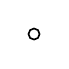
\begin{tikzpicture}
	\node[circle, draw, semithick, inner sep=0pt, minimum size=4pt] (1) at (0,0) {};
	\end{tikzpicture}
}

%----------------------------------------------------------------------------------------
%	TITLE PAGE
%----------------------------------------------------------------------------------------

\setbeamertemplate{title page}{%

	\begin{tikzpicture}[remember picture,overlay]
	
	% Uni logo
	\node[inner sep=0pt] (logo) at (1.1, 3)
	{
\includegraphics[width=.3\textwidth]{images/logo.pdf}};
	
	% Uni pic
	\node[inner sep=0pt] (logo) at (9.175, 1.62)
	{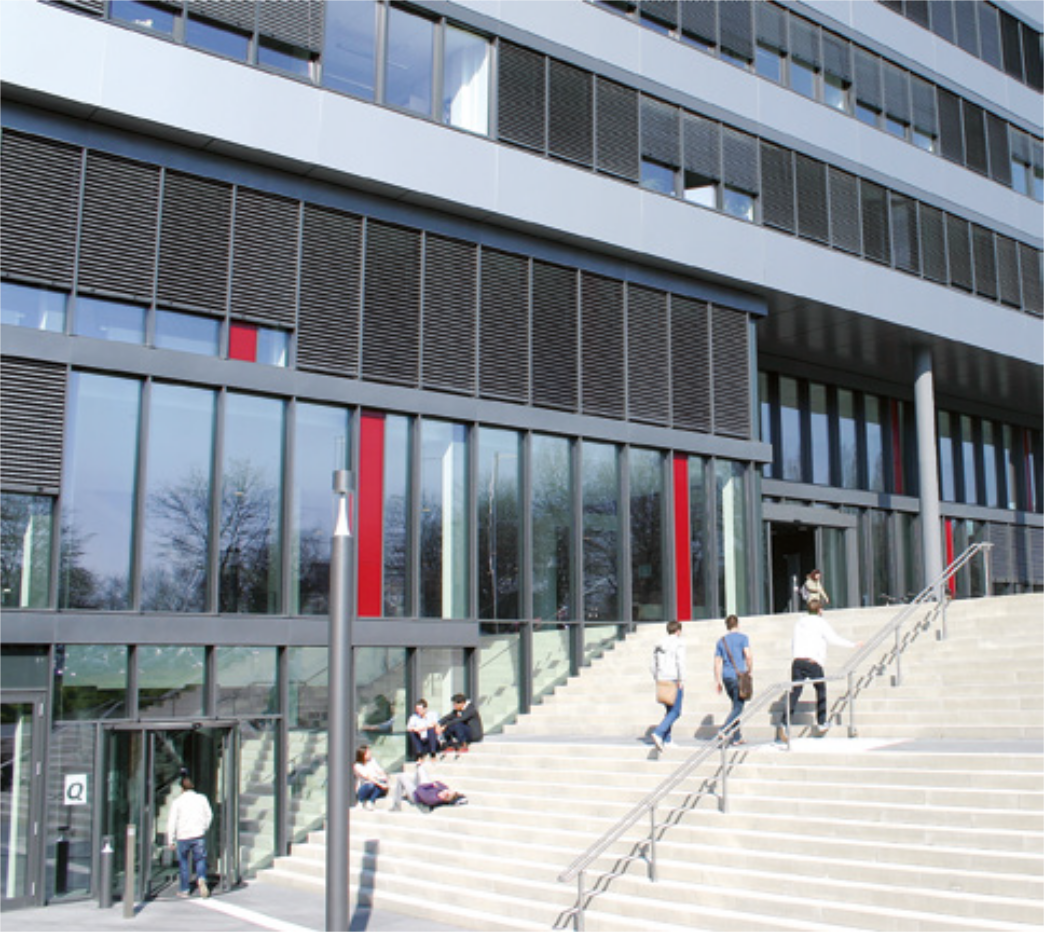
\includegraphics[width=.485\textwidth]{images/unibuilding.png}};
	

	\node[inner sep=0pt] (tit) at (4.40, -2.7)
	{
		\begin{minipage}[t]{1.0\linewidth} 
		\setbeamercolor{title}{bg=\upbcolor,fg=white}	
		
		\begin{minipage}[t]{1.0\linewidth} 
		\setbeamercolor{title}{bg=,fg=uni-blue}	
		\begin{beamercolorbox}[sep=2pt,left]{title}
		{\hspace{4pt}{\vspace{0.1cm}\fontsize{10}{16}\fontfamily{phv}\fontseries{bc}\selectfont\bfseries\insertinstitute}}
		\end{beamercolorbox}
		
		\end{minipage}  	
		
		\begin{minipage}{1.0\linewidth} 
		
		
		\begin{beamercolorbox}[sep=8pt,left]{title}
		
		{\lenitem{\fontsize{\upbtitlesize}{\upbtitlelinespace}\fontfamily{phv}\fontseries{mc}\selectfont\bfseries\color{white}\raggedright\inserttitle}}%
		
		\end{beamercolorbox}
		
		\end{minipage}  	
		
		\ifx\insertsubtitle\@empty%
		\else%
		{		\begin{minipage}[t]{0.9\linewidth} 
			\setbeamercolor{title}{bg=,fg=uni-blue}	
			\begin{beamercolorbox}[sep=4pt,left]{subtitle}
			{\hspace{4pt}\vspace{0.2cm}{\fontsize{10}{16}\fontfamily{phv}\fontseries{bc}\selectfont\bfseries \insertsubtitle}}
			\end{beamercolorbox}
			\end{minipage}  	
		}
		\fi%   			
		
		\end{minipage}  		
		
	};
	
	\end{tikzpicture}	
	
}

%----------------------------------------------------------------------------------------
%	FRAME TITLE THEME
%----------------------------------------------------------------------------------------

\setbeamertemplate{frametitle}
{
	\nointerlineskip
	
	\fontfamily{phv}\fontseries{bc}\selectfont\bfseries 
	\setbeamercolor{frametitle}{bg=,fg=\upbcolor}	
	
	\begin{beamercolorbox}[sep=0.3cm,ht=5.3em,wd=\paperwidth]{frametitle}
		\vbox{}\vskip-2ex%
		\hspace{0.05cm}
		
\includegraphics[width=1.8cm]{images/logo}
		\hfill
		\vskip1.2ex%
		\vspace{0.1cm}
		\hspace{0.0cm}
		\insertframetitle
	\end{beamercolorbox}
	\vspace{-0.4cm}
	
}

% Title
\title{Title Lorem ipsum dolor sit amet consectetur adipiscing elit Phasellus ac odio ex} 

% Sub Title
\subtitle{Subtitle goes here}

% Your name
\author{Ashwin Prasad Shivarpatna Venkatesh}

% Your institution for the title page
\institute{Institution name} 

% Date, can be changed to a custom date
\date{\today} 

% Choose primary UPB color for title, headings etc.. 
% Choose from 
% (uni-cyan, uni-black, uni-blue, uni-orange, uni-purple, uni-green)
\newcommand{\upbcolor}{uni-blue} 




%----------------------------------------------------------------------------------------
%	TITLE PAGE
%----------------------------------------------------------------------------------------


\begin{document}

{
\upbtitlebackground 
\begin{frame}
%\upblogo
\titlepage % Print the title page as the first slide
\end{frame}
}

\begin{frame}
\frametitle{Overview} % Table of contents slide, comment this block out to remove it
\tableofcontents % Throughout your presentation, if you choose to use \section{} and \subsection{} commands, these will automatically be printed on this slide as an overview of your presentation
\end{frame}

%----------------------------------------------------------------------------------------
%	PRESENTATION SLIDES
%----------------------------------------------------------------------------------------

%------------------------------------------------
\section{First Section} % Sections can be created in order to organize your presentation into discrete blocks, all sections and subsections are automatically printed in the table of contents as an overview of the talk
%------------------------------------------------

\subsection{Subsection Example} % A subsection can be created just before a set of slides with a common theme to further break down your presentation into chunks

\begin{frame}
\frametitle{Paragraphs of Text}

Paragraphs Sed iaculis dapibus gravida. Morbi sed tortor erat, nec interdum arcu. Sed id lorem lectus. Quisque viverra augue id sem ornare non aliquam nibh tristique. Aenean in ligula nisl. Nulla sed tellus ipsum. Donec vestibulum ligula non lorem vulputate fermentum accumsan neque mollis.\\~\\

Sed diam enim, sagittis nec condimentum sit amet, ullamcorper sit amet libero. Aliquam vel dui orci, a porta odio. Nullam id suscipit ipsum. 
\end{frame}

%------------------------------------------------

\begin{frame}
\frametitle{Bullet Points}
\begin{itemize}[<+->]
\item Lorem ipsum dolor sit amet, consectetur adipiscing elit
\begin{itemize}
\item Aliquam blandit faucibus nisi, sit amet dapibus enim tempus eu
\end{itemize}
\item Aliquam blandit faucibus nisi, sit amet dapibus enim tempus eu
\item Nulla commodo, erat quis gravida posuere, elit lacus lobortis est, quis porttitor odio mauris at libero
\item Nam cursus est eget velit posuere pellentesque
\item Vestibulum faucibus velit a augue condimentum quis convallis nulla gravida
\item Nam cursus est eget velit posuere pellentesque
\end{itemize}
\end{frame}

%------------------------------------------------

\begin{frame}[fragile]
\frametitle{Code Example}

	
	{
		
		\begin{lstlisting}[language=c,caption=C Code,basicstyle=\ttfamily,linebackgroundcolor={\ifnum\value{lstnumber}=2\color{uni-green}\else\color{white}\fi}]		
int cond_select(bool b, int x, int y){
	if(b){
		return x;
	} 
	else {
		return y;
	}
}
		\end{lstlisting}
		
	}
	
%------------------------------------------------

\end{frame}

\begin{frame}
\frametitle{Blocks of Highlighted Text}
\begin{block}{Block 1}
Lorem ipsum dolor sit amet, consectetur adipiscing elit. Integer lectus nisl, ultricies in feugiat rutrum, porttitor sit amet augue. Aliquam ut tortor mauris. Sed volutpat ante purus, quis accumsan dolor.
\end{block}

\begin{block}{Block 2}
Pellentesque sed tellus purus. Class aptent taciti sociosqu ad litora torquent per conubia nostra, per inceptos himenaeos. Vestibulum quis magna at risus dictum tempor eu vitae velit.
\end{block}

\end{frame}

%------------------------------------------------

\begin{frame}
\frametitle{Multiple Columns}
\begin{columns}[c] % The "c" option specifies centered vertical alignment while the "t" option is used for top vertical alignment

\column{.45\textwidth} % Left column and width
\textbf{Heading}
\begin{enumerate}
\item Statement
\item Explanation
\item Example
\end{enumerate}

\column{.5\textwidth} % Right column and width
\begin{figure}
	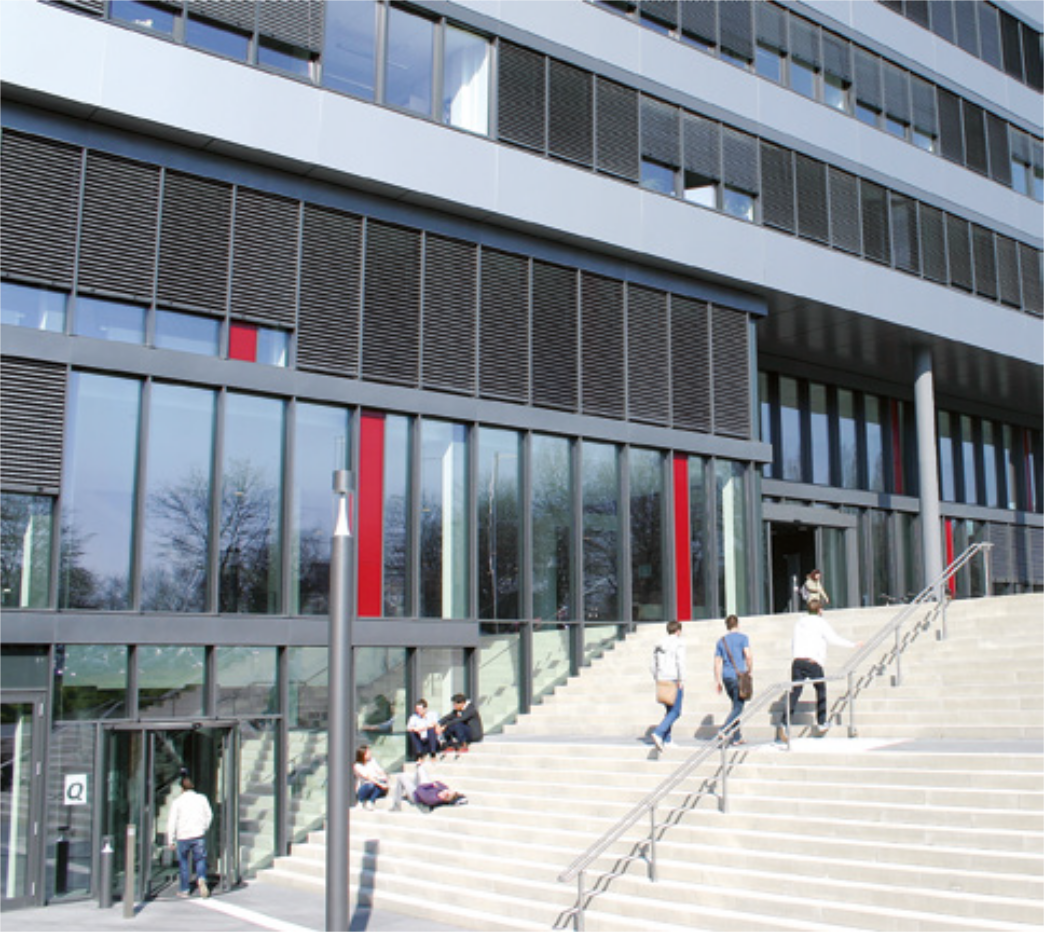
\includegraphics[width=1\textwidth]{images/unibuilding.png}
\end{figure}


\end{columns}
\end{frame}

%------------------------------------------------
\section{Second Section}
%------------------------------------------------

\begin{frame}
\frametitle{Table}
\begin{table}
\begin{tabular}{l l l}
\toprule
\textbf{Treatments} & \textbf{Response 1} & \textbf{Response 2}\\
\midrule
Treatment 1 & 0.0003262 & 0.562 \\
Treatment 2 & 0.0015681 & 0.910 \\
Treatment 3 & 0.0009271 & 0.296 \\
\bottomrule
\end{tabular}
\caption{Table caption}
\end{table}
\end{frame}

%------------------------------------------------

\begin{frame}
\frametitle{Theorem}
\begin{theorem}[Mass--energy equivalence]
$E = mc^2$
\end{theorem}
\end{frame}

%------------------------------------------------

\begin{frame}
\frametitle{Figure}
Change the location on this slide to include your own image from the images directory found on the same directory as the template .TeX file. Can also include overlay image in the second frame of this slide.
\begin{figure}

\includegraphics[width=0.8\linewidth]{images/logo.pdf}
\end{figure}

\begin{onlyenv}<2>
	%\begin{tikzpicture}[remember picture,overlay]
	%\node[drop shadow={shadow xshift=.8ex,shadowyshift=-.8ex},fill=white,draw] at (0,0) {\includegraphics[width=12cm]{images/deadstoreex}};
	%%\node at (current page.center) {\includegraphics[width=12cm]{images/deadstoreex}};
	%
	%
	%\end{tikzpicture}
	
	\begin{tikzpicture}[remember picture,overlay]
	\node[drop shadow={shadow xshift=.8ex,shadow yshift=-.8ex},fill=white,draw] at (current page.center) {
\includegraphics[width=11cm]{images/logo.pdf}};
	\end{tikzpicture}
	
\end{onlyenv}
\end{frame}




%------------------------------------------------

\begin{frame}[fragile] % Need to use the fragile option when verbatim is used in the slide
\frametitle{Citation}
An example of the \verb|\cite| command to cite within the presentation:\\~

This statement requires citation \cite{p1}.
\end{frame}

%------------------------------------------------

\begin{frame}
\frametitle{References}
\footnotesize{
\begin{thebibliography}{99} % Beamer does not support BibTeX so references must be inserted manually as below
\bibitem[Smith, 2012]{p1} John Smith (2012)
\newblock Title of the publication
\newblock \emph{Journal Name} 12(3), 45 -- 678.
\end{thebibliography}
}
\end{frame}

%------------------------------------------------

\begin{frame}
\Huge{\centerline{The End}}
\end{frame}

%----------------------------------------------------------------------------------------

\end{document} 